\subsection{Descripci\'on del problema}

Este problema conciste en generar la silueta de una ciudad a partir de la representacion de varios edificios que la componen.
A la entrada del algoritmo voy a tener una cantidad textbf{N} de edificios, representados con tres valores; en donde comienza, su altura y dode termina. Todos los valores son enteros positivos, en relacion los texttt{ceros} de cada eje, horizontal y longitudinal.
A la salida voy a tener representada la silueta de la ciudad como una seguidillas de puntos que representan el contorno de los edificios que textbf{sobresalen} del resto.
La gracia de todo esto es ocultar las partes de los edificios que quedan textbf{dentro} de otros edificios.

\subsubsection*{Escenarios t\'ipicos}
\addcontentsline{toc}{subsubsection}{Escenarios t\'ipicos}

Las siguientes instancias son las b\'asicas a las cuales se pueden reducir todos los escenarios.

\subsubsection*{Edificio B\'asico}
\addcontentsline{toc}{subsubsection}{Edificio B\'asico}
\begin{figure}[H]
\begin{center}
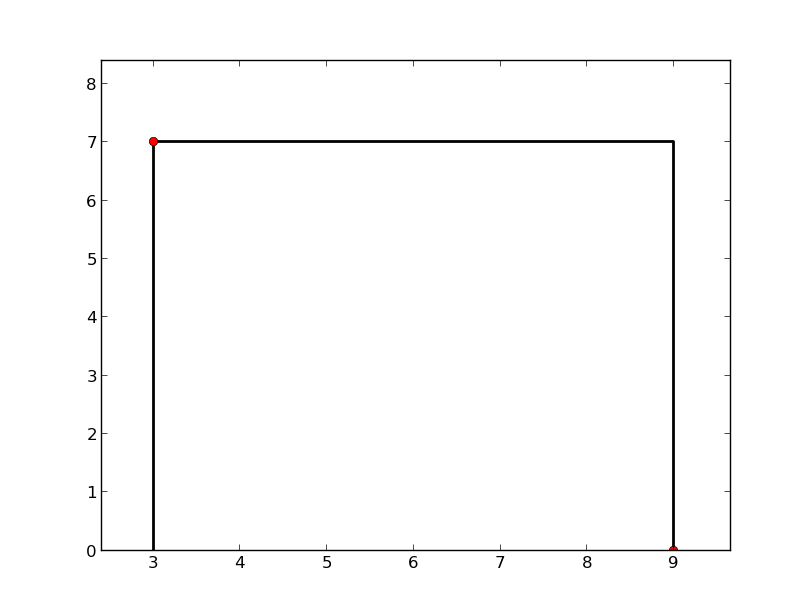
\includegraphics[scale=0.5]{./imagenes/ej2_edificio1.png}
\caption{Un solo edificio con los puntos que serian la representaci\'on de su silueta}
\end{center}
\end{figure}
\begin{figure}[H]
\begin{center}
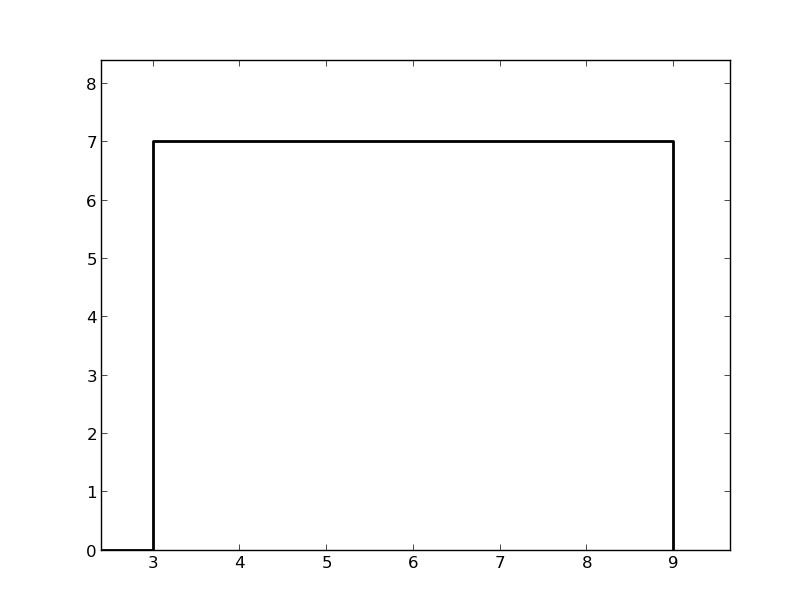
\includegraphics[scale=0.5]{./imagenes/ej2_edificio1solucion.png}
\caption{La ciudad que representa un solo edificio}
\end{center}
\end{figure}


\subsubsection*{Edificios Cruzados 1}
\addcontentsline{toc}{subsubsection}{Edificios Cruzados 1}
\begin{figure}[H]
\begin{center}
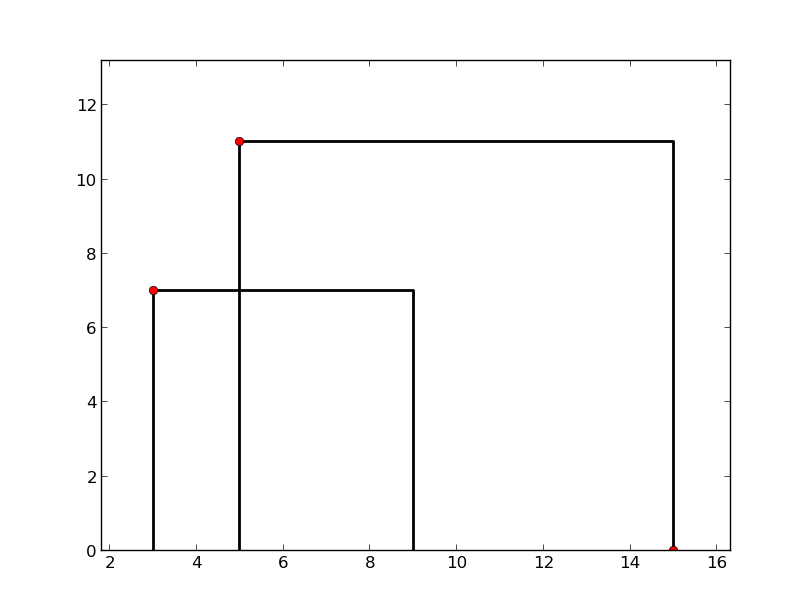
\includegraphics[scale=0.5]{./imagenes/ej2_edificio2.png}
\caption{Edificios Cruzados 1}
\end{center}
\end{figure}
\begin{figure}[H]
\begin{center}
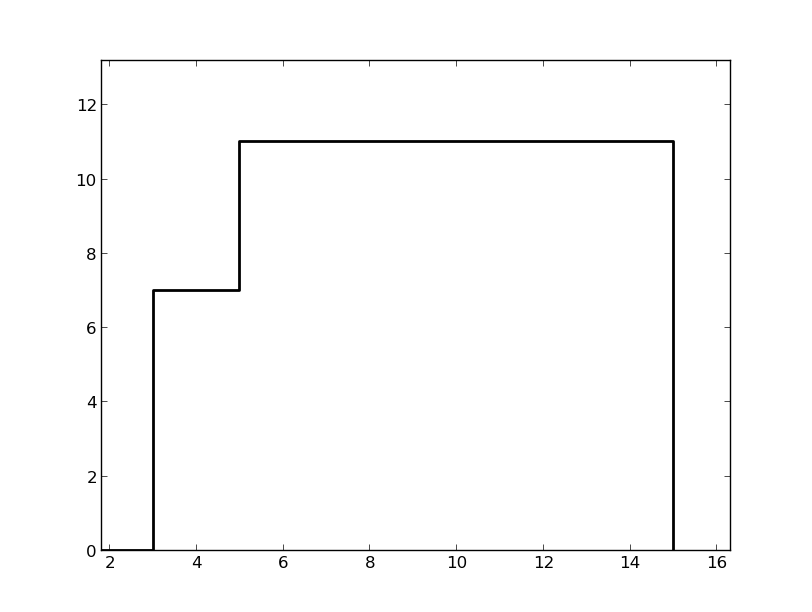
\includegraphics[scale=0.5]{./imagenes/ej2_edificio2solucion.png}
\caption{Silueta representado la ciudade de edificios cruzados 1}
\end{center}
\end{figure}

\subsubsection*{Edificios Cruzados 2}
\addcontentsline{toc}{subsubsection}{Edificios Cruzados 2}
\begin{figure}[H]
\begin{center}
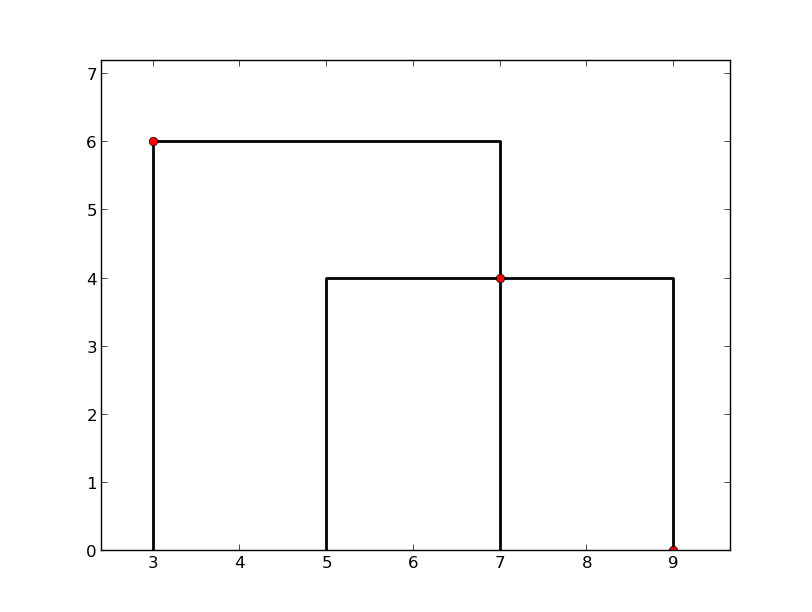
\includegraphics[scale=0.5]{./imagenes/ej2_edificio3.png}
\caption{Edificios cruzados}
\end{center}
\end{figure}
\begin{figure}[H]
\begin{center}
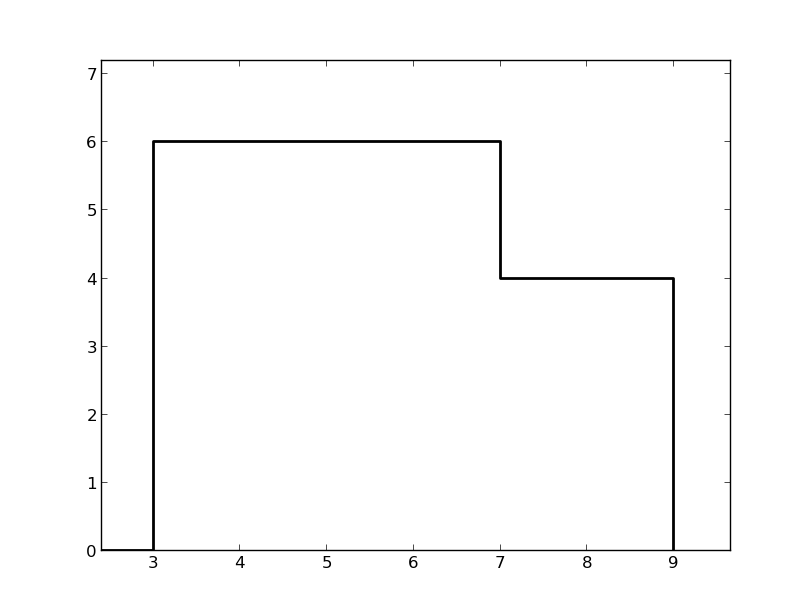
\includegraphics[scale=0.5]{./imagenes/ej2_edificio3solucion.png}
\caption{Silueta representado la ciudade de edificios cruzados 1}
\end{center}
\end{figure}

\subsubsection*{Edificios Solapados}
\addcontentsline{toc}{subsubsection}{Edificios Solapados}
\begin{figure}[H]
\begin{center}
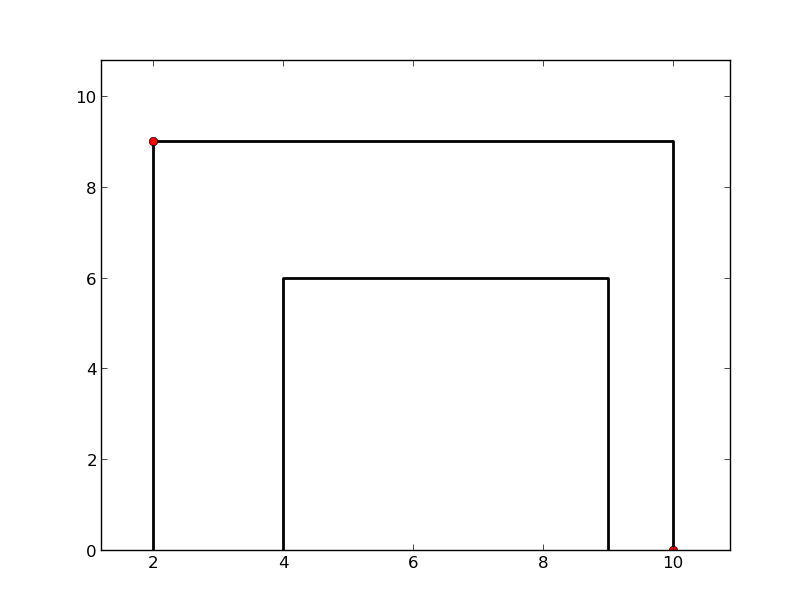
\includegraphics[scale=0.5]{./imagenes/ej2_edificio4.png}
\caption{Un edificio dentro del otro}
\end{center}
\end{figure}
\begin{figure}[H]
\begin{center}
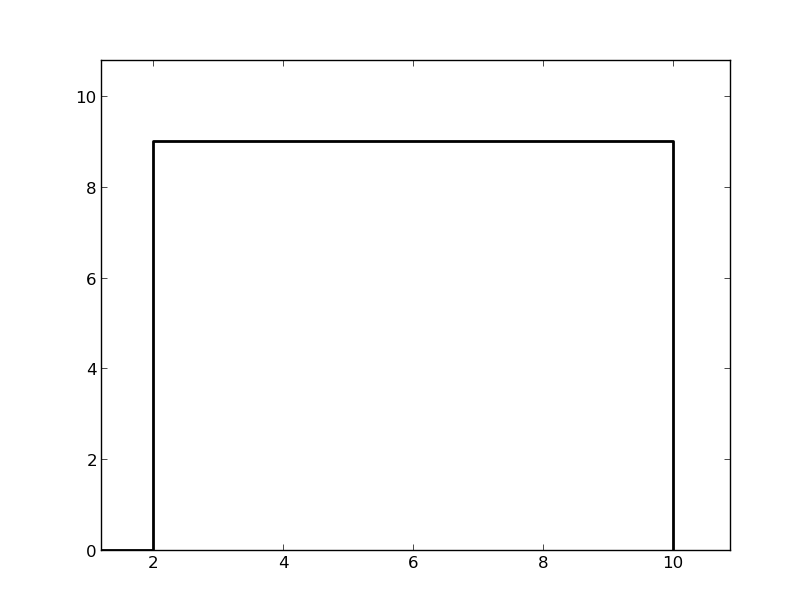
\includegraphics[scale=0.5]{./imagenes/ej2_edificio4solucion.png}
\caption{La ciudad es la silueta del edificio m\'as grande que opaca/absorbe al m\'as peque\'no'}
\end{center}
\end{figure}

\subsubsection*{Edificios Contiguos}
\addcontentsline{toc}{subsubsection}{Edificios Contiguos}
\begin{figure}[H]
\begin{center}
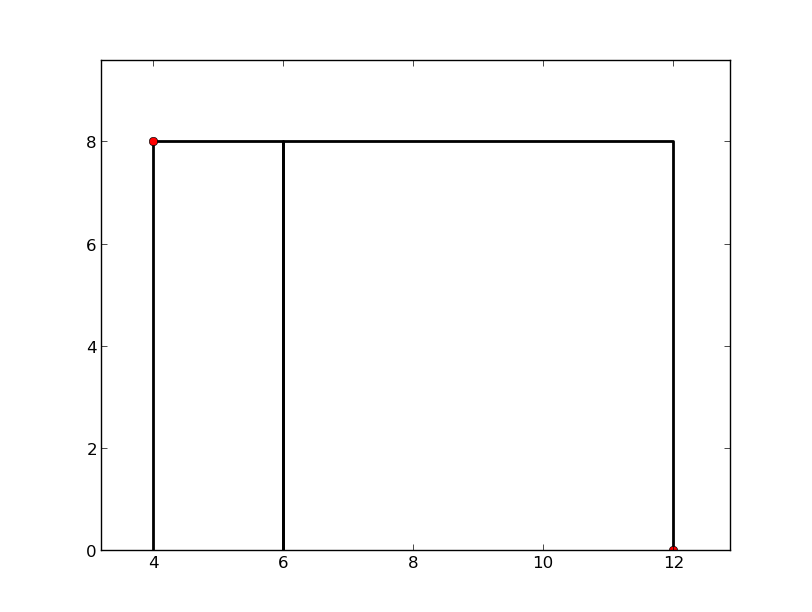
\includegraphics[scale=0.5]{./imagenes/ej2_edificio5.png}
\caption{Dos edificios contiguos de la misma altura}
\end{center}
\end{figure}
\begin{figure}[H]
\begin{center}
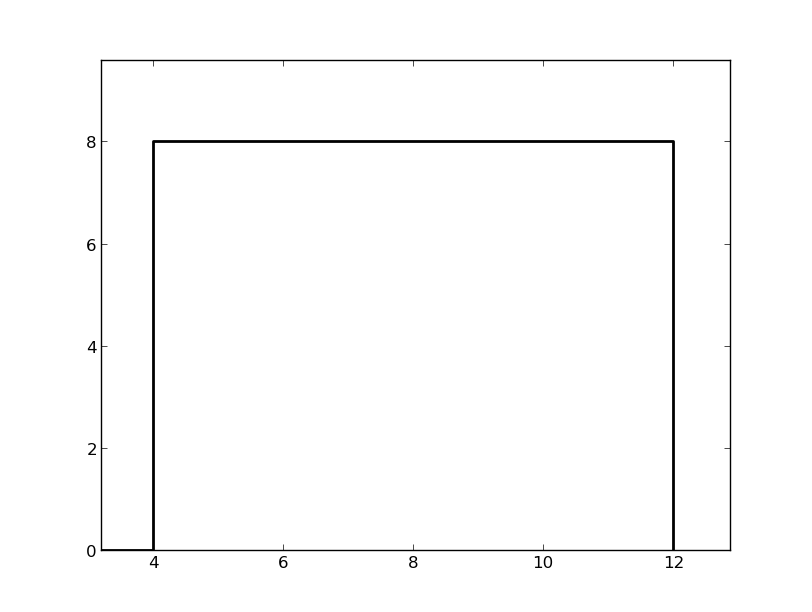
\includegraphics[scale=0.5]{./imagenes/ej2_edificio5solucion.png}
\caption{La ciudad, que es la suma de los dos edificios, ya que estan pegados.}
\end{center}
\end{figure}



\subsection{Resoluci\'on}


\subsection{Demostraci\'on de la resoluci\'on}


\subsection{Complejidad del algoritmo}


\subsection{C\'odigo fuente}

\lstset{language=C++,
                basicstyle=\ttfamily\footnotesize,
                keywordstyle=\color{blue}\ttfamily,
                stringstyle=\color{red}\ttfamily,
                commentstyle=\color{green}\ttfamily,
                morecomment=[l][\color{magenta}]{\#},
                breaklines=true
}
\begin{lstlisting}


\end{lstlisting}

\subsection{Casos de prueba}

\subsection{Performance}
